\section{3G}

3G modulet testes som et selvstændigt modul. 
Testene der udføres er PUT og GET, da det er disse metoder der er implementeret på dronen. 
For at udføre tests med 3G modulet, kræves en fungerende server der tillader HTTP requests. Projektets webserver anvendes ikke til testen, for kun at have fokus på en enhed. Istedet er hjemmesiden requestb.in[X] anvendt, da requestb.in tillader HTTP kommunikation. Ved Requestb.in får man en URL, denne URL anvendes til både PUT og GET requests.

På figur \ref{fig:get_req} vises et GET request til en requestb.in server. I dette tilfælde: requestb.in/1d8w2501. Den første linje efter \textit{data:} fortæller om requestet er gennemført succesfuldt eller om der er sket en fejl. Svaret 200 ok betyder at requestet er gået igennem og det ønskede data er hentet. 

\begin{figure}[H]
\centering
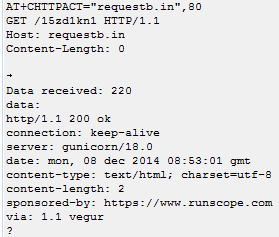
\includegraphics[width=0.5\textwidth]{Billeder/Test/get_requestbin.png}
\caption{GET Request}
\label{fig:get_req}
\end{figure}

Ved brug af PUT, opdateres information der allerede ligger på serveren. Figur \ref{fig:putrequest_module} viser hvad der sendes til serveren. Det information der er sendt, er tilgængelig på serveren, som vist på figur \ref{fig:put_req}.

\begin{figure}[H]
\centering
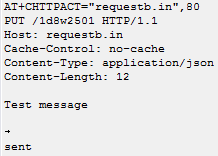
\includegraphics[width=0.5\textwidth]{Billeder/Test/putrequest_module.png}
\caption{PUT metode}
\label{fig:putrequest_module}
\end{figure}

RAW BODY viser dataet der er sendt og HEADERS indeholder parametrene for HTTP protokollen.

\begin{figure}[H]
\centering
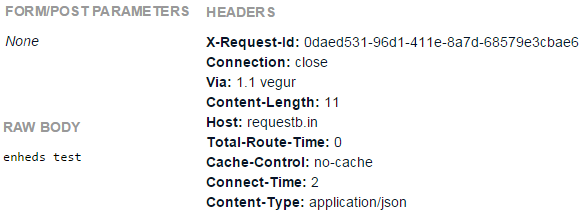
\includegraphics[width=0.8\textwidth]{Billeder/Test/put_request.png}
\caption{Information på server}
\label{fig:put_req}
\end{figure}
